\documentclass[10pt, compress]{beamer}

\usetheme{m}
\usepackage{amssymb}
\usepackage{graphicx}
\usepackage{booktabs}
\usepackage[scale=2]{ccicons}
\usepackage{minted}
\usemintedstyle{perldoc}

\usepgfplotslibrary{dateplot}

\usemintedstyle{trac}

\usepackage{datetime}
\newdate{date}{06}{08}{2015}

\usepackage{verbatim}
\usepackage{tikz}

\title{Quantitative Methods for Surveys}
\subtitle{Master’s in Sustainability Leadership,\\
Cambridge Institute for Sustainability Leadership}
\date{\displaydate{date}}
\author{Sreekumar Thaithara Balan}
\institute{Department of Physics and Astronomy,\\
University College London\\
sbalan@star.ucl.ac.uk}

\begin{document}

\maketitle

\section{Objectives}

\begin{frame}[t]{Objectives}
    \begin{itemize}
        \item What are surveys?
        \item Concept of sampling
        \item Sampling error and non-sampling error
        \item Probability and non-probability samples
        \item Inferences from the data
    \end{itemize}
\end{frame}
%--- Next Frame ---%


\section{Outline}

\begin{frame}
    \frametitle{Outline}
    \begin{itemize}
        \item Introduction to survyes
        \item Survey sampling
        \item Describing and making inferences from the data
    \end{itemize}
\end{frame}

\section{Introduction to surveys}

\begin{frame}
    \frametitle{Basic idea of a survey}
    \begin{itemize}
        \item collect quantitative information
        \item answering a questionnaire
        \item interviewes by a researcher
    \end{itemize}
\end{frame}

% http://www.custominsight.com/articles/collecting-survey-data.asp
\begin{frame}
    \frametitle{Where do we start?}
    \begin{block}{Before we begin...}
        \begin{itemize}
            \item you \alert{MUST} take the time to really understand the purpose of your survey
            \item you need to keep this purpose in mind every step of the way
        \end{itemize}
    \end{block}
\end{frame}

\begin{frame}
    \frametitle{What would you like to know?}
    \begin{enumerate}
        \item Is there already an existing survey template that has statistically validated and proven survey questions?
        \item Mentally walk through the steps you will take once the data have been collected. What do you expect to learn? How do you plan to apply what you learn?
        \item Inputs from other people / sources will be very useful
        \item What issues relate to each topical area of your survey?
        \item Construct an outline of the issues and details that you collected in steps 1 and 2.
    \end{enumerate}
\end{frame}

% https://scholar.vt.edu/access/content/group/43c8db00-e78f-4dcd-826c-ac236fb59e24/STAT3615/Sampling%20and%20Observational%20Studies.htm
\begin{frame}
    \frametitle{Research Strategies}
    \begin{block}{Observational Studies}
        \begin{itemize}
            \item Purpose is to learn about some large population
            \item Representative sample (subgroup) chosen at random from the population for study (questioning or examination)
            %\item No intervention, manipulation, or treatment
            \item Conclusions drawn about the sample generalized to population
            \item Results do \alert{not} imply cause and effect
        \end{itemize}
    \end{block}
    \begin{block}{Experiments}
        \begin{itemize}
            \item Purpose is to measure the effect of an explanatory variable on the response or outcome variable
            \item explanatory variable = an intervention, manipulation, or treatment applied to the experimental unit
            \item Results do imply cause and effect (if done properly)
        \end{itemize}
    \end{block}
\end{frame}


\begin{frame}
    \frametitle{Terms in Survey Sampling}
    % http://www.slideshare.net/drkellypage/pagek-marketing-researchwk61?next_slideshow=1
    \begin{columns}
        \column{0.5\textwidth}
        \begin{block}{}
            \begin{itemize}
                \item population : Entire group of people about whom information
                is required.
                \item census : Collection of data from or about every member of
                the population.
                \item sample : Subset of all members of a population of interest
                \item sampling frame : List of population elements from which
                units to be sampled cab be selected.
                \item sample survey
            \end{itemize}
        \end{block}
        \column{0.5\textwidth}
        \begin{block}{}
            \begin{figure}
                \begin{center}
                    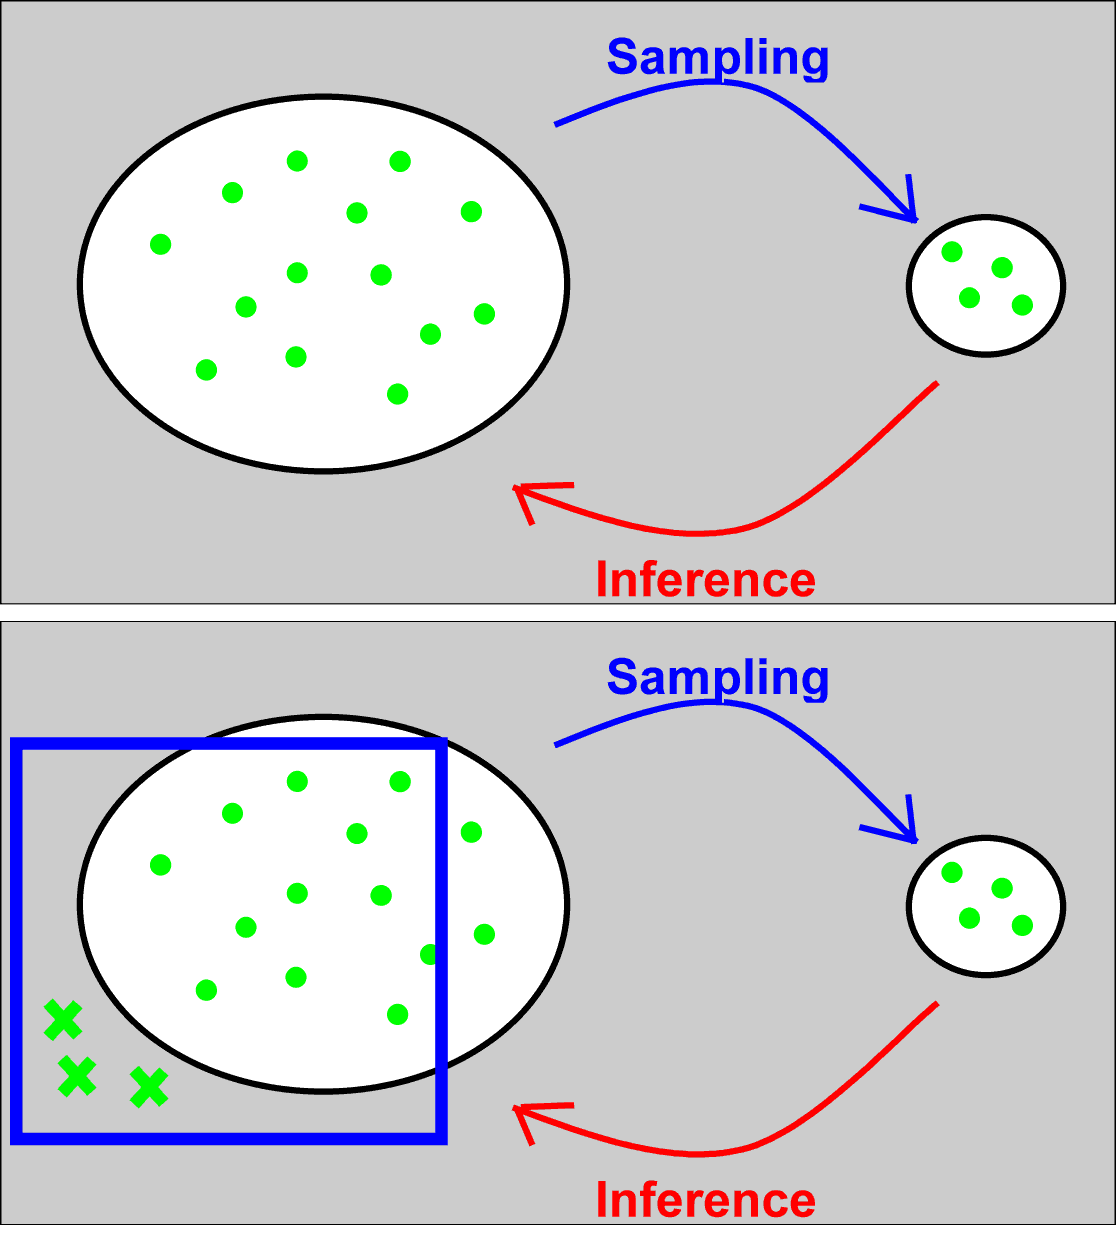
\includegraphics[scale=0.1]{img/PopulationFrame.png}
                \end{center}
            \end{figure}
        \end{block}
    \end{columns}
\end{frame}

\begin{frame}
    \frametitle{Characterstics of a good sample}
    % http://www.slideshare.net/ReaNoel/sampling-111121003751phpapp01
    \begin{itemize}
        \item Representativeness
        \item Unbiasedness
        \item Precision
        \item Adequate in size
    \end{itemize}
\end{frame}

\begin{frame}
    \frametitle{Limitations of Sampling}
    \begin{itemize}
        \item Results may be incorrect or misleading
        \item Representativeness may not be achieved
    \end{itemize}
\end{frame}

\begin{frame}[t]{Developing a sampling design}
    \begin{itemize}
        \item Define the population of interest
        \item Choose data collection method
        \item Indentify sampling frame
        \item Select Sampling method
        \item Determine the sample size
    \end{itemize}
\end{frame}
%--- Next Frame ---%

\begin{frame}[t]{Population of interest}
    \begin{itemize}
        \item Think about possible bases of defining a population
        \item e.g., Geographical area, demographic (age, gender, etc.)
        \item Do you need to apply any filter?
    \end{itemize}
\end{frame}
%--- Next Frame ---%

\begin{frame}[t]{Data collection method}
    % http://www.slideshare.net/drkellypage/pagek-marketing-researchwk61?next_slideshow=1
    \begin{itemize}
        \item What methods can be used to reach the population of interest?
        \item What methods can be used to administer the survey?
        \item What are the resource implications?
        \item What are the implications regarding the representativess of the survey?
    \end{itemize}
\end{frame}
%--- Next Frame ---%

\begin{frame}[t]{Indentify the sampling frame}
    % http://www.slideshare.net/drkellypage/pagek-marketing-researchwk61?next_slideshow=1
    \begin{itemize}
        \item Listings
        \begin{itemize}
            \item Electoral register
            \item Postcode address file
            \item Telephone directory
            \item Consumer lists
            \item Employee lists
        \end{itemize}
        \item Think about
        \begin{itemize}
            \item Who is excluded?
            \item How could this affect the representativeness?
        \end{itemize}
        \item There may by no exsisting sampling frame. You will have to formulate a plan.
    \end{itemize}
\end{frame}
%--- Next Frame ---%

\begin{frame}[t]{Select a sampling method}
    % https://scholar.vt.edu/access/content/group/43c8db00-e78f-4dcd-826c-ac236fb59e24/STAT3615/Sampling%20and%20Observational%20Studies.htm
    \begin{itemize}
        %\item Poor sampling designs
        \item Probability Sampling
        \item Non-Probability Sampling
    \end{itemize}
\end{frame}
%--- Next Frame ---%

\begin{frame}[t]{Let us pause for a minute...}
    \begin{itemize}
        \item Research question
        \item Population
        \item Sampling frame
        \item Data collection
    \end{itemize}
    \bigskip
    Now we can move on to sampling designs...
\end{frame}
%--- Next Frame ---%


\begin{frame}[t]{Probability Sampling}
    \begin{itemize}
        \item Simple random sampling
        \item Stratified random sampling
        \item Cluster sampling
        \item Systematic sampling
        \item Random digit dialing
        \item Multi-stage sampling
    \end{itemize}
\end{frame}
%--- Next Frame ---%

\begin{frame}[t]{Simple random sampling}
    \begin{columns}
        \column{0.5\textwidth}
        \begin{block}{}
            \begin{itemize}
                \item Each unit of the population has equal chance of being included in the sample.
                \item Every combination of $n$ units of the population has the same chance of being included in the sample of size $n$.
                \item Usually accomplished by mixing the population and taking a sample of size $n$
                \item requires the full list of population of interest
                \item we may use a random number generator to pick the units
            \end{itemize}
        \end{block}
        \column{0.5\textwidth}
        \begin{block}{}
            \begin{figure}
                \begin{center}
                    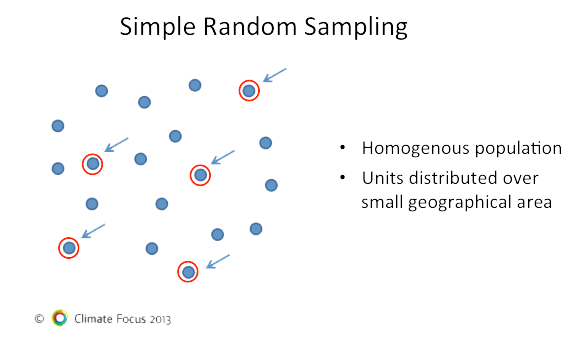
\includegraphics[scale=0.25]{img/Slide2.png}
                \end{center}
            \end{figure}
        \end{block}
    \end{columns}
\end{frame}
%--- Next Frame ---%

\begin{frame}[t]{Stratified random sampling}
    \begin{columns}
        \column{0.5\textwidth}
        \begin{block}{}
            \begin{itemize}
                \item The population is divided into strata
                \item A simple random sample is taken from each strata
                \item e.g., U.S. by State, Cambridge Students by College
                \item mutually exclusive and exhasutive groups
                \item reduces the sampling error
                \item proportional allocation
                \item weighting the sample
            \end{itemize}
        \end{block}
        \column{0.5\textwidth}
        \begin{block}{}
            \begin{figure}
                \begin{center}
                    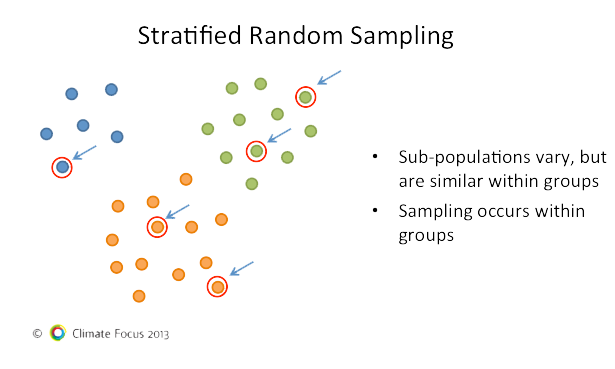
\includegraphics[scale=0.25]{img/Slide3.png}
                \end{center}
            \end{figure}
        \end{block}
    \end{columns}

\end{frame}
%--- Next Frame ---%

\begin{frame}[t]{Cluster sampling}
    \begin{columns}
        \column{0.5\textwidth}
        \begin{block}{}
            \begin{itemize}
                \item Randomizing the units within the population is not feasible
                \item Random clusters of individuals are sampled, but cluster membership is not at random
                \item Each individual in the cluster is observed/measure
                \item divides the population area into sections (clusters) then randomly selects clusters and chooses all the members of those clusters
            \end{itemize}
        \end{block}
        \column{0.5\textwidth}
        \begin{block}{}
            \begin{figure}
                \begin{center}
                    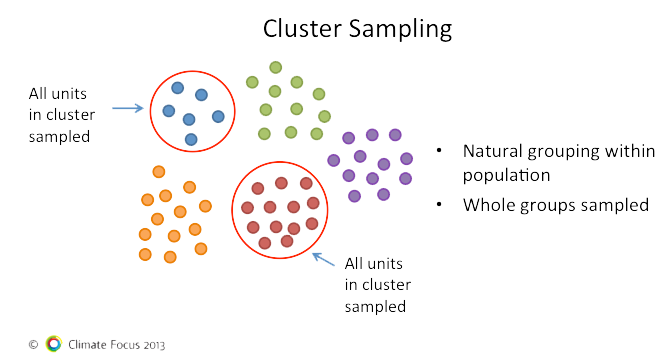
\includegraphics[scale=0.25]{img/Slide5.png}
                \end{center}
            \end{figure}
        \end{block}
    \end{columns}

\end{frame}
%--- Next Frame ---%

\begin{frame}[t]{Systematic sampling}
    \begin{columns}
        \column{0.5\textwidth}
        \begin{block}{}
            \begin{itemize}
                \item Population is ordered
                \item Every k-th unit is sampled, e.g., every 10th or every 50th
            \end{itemize}
        \end{block}
        \column{0.5\textwidth}
        \begin{block}{}
            \begin{figure}
                \begin{center}
                    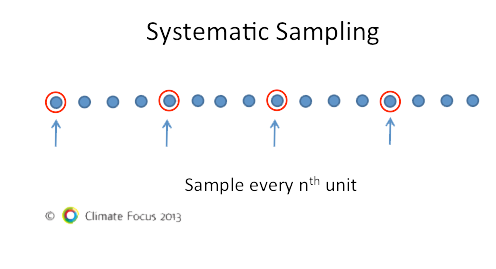
\includegraphics[scale=0.25]{img/Slide4.png}
                \end{center}
            \end{figure}
        \end{block}
    \end{columns}

\end{frame}
%--- Next Frame ---%

\begin{frame}[t]{Multi-stage sampling}
    \begin{columns}
        \column{0.5\textwidth}
        \begin{block}{}
            \begin{itemize}
                \item sequential combinations of the above sampling plans.
                \item Multi-stage Sampling is a more complex form of Cluster Sampling
                \item not all the units within a sub-group need to be measured. Instead, samples of sub-group units are measured
            \end{itemize}
        \end{block}
        \column{0.5\textwidth}
        \begin{block}{}
            \begin{figure}
                \begin{center}
                    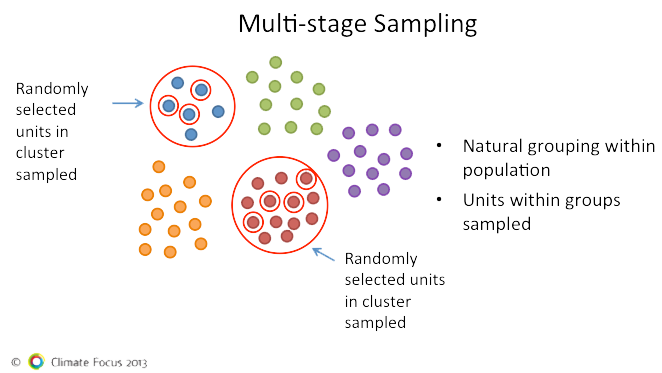
\includegraphics[scale=0.25]{img/Slide6.png}
                \end{center}
            \end{figure}
        \end{block}
    \end{columns}

\end{frame}
%--- Next Frame ---%

\begin{frame}[t]{Statistical Accuracy - Confidence and Error}
    % http://www.custominsight.com/articles/random-sampling.asp
    \begin{itemize}
        \item Error - This is that ``plus or minus X\%'' that you hear about. What it means is that you feel confident that your results have an error of no more than X\%.
        \item Confidence - This is how confident you feel about your error level. Expressed as a percentage, it is the same as saying if you were to conduct the survey multiple times, how often would you expect to get similar results.
    \end{itemize}
    \smallskip
    These two concepts work together to determine how accurate your survey results are. For example, if you have 90\% confidence with an error of 4\%, you are saying that if you were to conduct the same survey 100 times, the results would be within $\pm$ 4\% of the first time you ran the survey 90 times out of 100.
\end{frame}
%--- Next Frame ---%

\begin{frame}[t]{Determining the ``Correct'' Sample Size}
    % http://www.custominsight.com/articles/random-sampling.asp
    Determining the ``correct'' sample size requires 3 pieces of information
    \begin{itemize}
        \item The size of your population
        \item Your desired error level (e.g. 5\%)
        \item Your desired level of confidence (e.g. 95\%)
    \end{itemize}
    %\url{http://www.custominsight.com/articles/random-sample-calculator.asp}
\end{frame}
%--- Next Frame ---%

%\begin{frame}[t]{Performing a Stratified Random Sample}
%    \begin{itemize}
%        \item Determine the size of the smallest subgroup in your population. For example, if you want to look at males vs. females and there are fewer females, then this is the group you want to look at.
%        \item Calculate the number of people required to achieve your desired error level and level of confidence for this subgroup.
%        \item Calculate what percentage of people that you will need to survey within this subgroup (number of people to survey divided by total subgroup size).
%        \item Finally, calculate the number of people in each of the other subgroups that are needed to achieve this same ratio (multiply the percentage from step 3 by the size of each of the other subgroups). This is how many people you will need to survey within each group.
%    \end{itemize}
%\end{frame}
%--- Next Frame ---%

\begin{frame}[t]{Non-probability sampling}
    \begin{itemize}
        \item Quota Sampling
        \item Conveniance Sampling
        \item Judgement Sampling
        \item Snowball Sampling
    \end{itemize}
\end{frame}
%--- Next Frame ---%

\begin{frame}[t]{Quota sampling}
    % http://www.slideshare.net/drkellypage/pagek-marketing-researchwk61?next_slideshow=1
    \begin{itemize}
        \item Very commonly used
        \item Population is devied into subgroups based on demographic crieteria,
        so that propotion of sample in each subgroup mirrors the popultaion of the
        subgroup in population.
        \item E.g., if the population of interest is 40\% male and 60\% female,
        the quota for the sample 500 repondents will tbe 200 males and 300 females
        \item Differs from startified random sampling.
        \item E.g., the demographic subroups are not necessarily related to the
        research question
        \item Selection of respondents is left to the researcher.
    \end{itemize}
\end{frame}
%--- Next Frame ---%

\begin{frame}[t]{Poor sampling designs}
    \begin{block}{Poor sampling designs $\Rightarrow$ bias}
        \begin{itemize}
            \item Convenience Sampling
            \begin{itemize}
                \item Using respondents how are willing
                \item A sample based on using people who are easiliy accessible
                such as mail intercepts or other high tracfic locations
                \item may save time and cost
            \end{itemize}
            \item Judgement Sampling
            \begin{itemize}
                \item Selection based on the judgement of the researcher
            \end{itemize}
            \item Snowball Sampling
            \begin{itemize}
                \item Select initial respondents and ask them to nominate others
            \end{itemize}
        \end{itemize}
    \end{block}
    \begin{block}{Bias}
        The design of a statistical study is biased if it systematically favors certain outcomes.
    \end{block}
\end{frame}
%--- Next Frame ---%

\begin{frame}[t]{Probability- or Non-Prbability-Sampling?}
    % http://www.slideshare.net/krishna1988/sampling-techniques-market-research
    \begin{table}
        \centering
        \begin{tabular}{|c|c|c|}
            \hline
            Factors & Non-Probaility & Probaility \\
            \hline
            \hline
            Nature of research & Exploratory & Conclusive \\
            larger magniture of & Non-Sampling errors & Sampling errors \\
            Variability & Homogeneous (low) & Hectrogeneous (large) \\
            Statistical traits & Unfavourable & Favourable \\
            Operational traits & Favourable & Unfavourable \\
            \hline
        \end{tabular}
    \end{table}
\end{frame}
%--- Next Frame ---%

\begin{frame}[t]{Selecting sampling method}
    Consider
    \begin{itemize}
        \item Nature of the research problem
        \item Objectives of the survey
        \item Time
        \item Budget
        \item Resource constraints
    \end{itemize}
\end{frame}
%--- Next Frame ---%

\begin{frame}[t]{More information}
    \begin{enumerate}
        \small
        \item \url{http://lc.gcumedia.com/hlt362v/the-visual-learner/the-visual-learner-v2.1.html}
        \item  \url{http://carbonfinanceforcookstoves.org/implementation/certification-process/monitoring-and-evaluation/}
        %\item \url{https://scholar.vt.edu/access/content/group/43c8db00-e78f-4dcd-826c-ac236fb59e24/STAT3615/Sampling%20and%20Observational%20Studies.htm}
        \item \url{http://www.slideshare.net/drkellypage/pagek-marketing-researchwk61}
    \end{enumerate}
\end{frame}
%--- Next Frame ---%


\end{document}
